% answers.tex —— 2018 年·北京卷·文科 · 参考答案与详细解析片段
% 由 tools/generate_projects.py 依来源总账自 2018/2018_数学真题_北京卷文_试题.md + 2018/2018_数学真题_北京卷文_解析正文.md + 2018/2018_数学真题_北京卷文_答案要点.md 生成，勿手改（改源 MD 后重跑）


\begin{gktip}
\textbf{来源与结论状态}：固定源仅有试题，没有答案或解析。以下解答为本库非官方推导，经过交叉复算，不代表官方答案。第9题固定源缺等号，条件性结论单独标明。
\end{gktip}

\gkpart{一、选择题}

\begin{answer}
\gksolhead{1}{}

\textbf{题目}：

已知集合 $A=\{x\mid |x|<2\}$，$B=\{-2,0,1,2\}$，则 $A\cap B=$\mbox{（　　）}

（A）$\{0,1\}$　（B）$\{-1,0,1\}$　（C）$\{-2,0,1,2\}$　（D）$\{-1,0,1,2\}$

\Needspace{4\baselineskip}
\textbf{解析}

\Needspace{5\baselineskip}
由 $|x|<2$ 得 $A=(-2,2)$。集合 $B$ 中只有 $0,1$ 严格落在该区间内，因此
\nopagebreak[4]
\[
A\cap B=\{0,1\}.
\]

\gkanswer{答案：A}

\end{answer}
\begin{answer}
\gksolhead{2}{}

\textbf{题目}：

在复平面内，复数 $\dfrac{1}{1-\mathrm i}$ 的共轭复数对应的点位于\mbox{（　　）}

（A）第一象限　（B）第二象限　（C）第三象限　（D）第四象限

\Needspace{4\baselineskip}
\textbf{解析}

\nopagebreak[4]
\[
\frac1{1-\mathrm i}=\frac{1+\mathrm i}{(1-\mathrm i)(1+\mathrm i)}=\frac{1+\mathrm i}{2}.
\]
其共轭复数为 $(1-\mathrm i)/2$，实部为正、虚部为负，对应点在第四象限。

\gkanswer{答案：D}

\end{answer}
\begin{answer}
\gksolhead{3}{}

\textbf{题目}：

执行如图所示的程序框图，输出的 $s$ 值为\mbox{（　　）}
\nopagebreak[4]
\begin{center}% 2018 北京卷文第3题：程序框图（据固定源第1063页重绘）
\begin{tikzpicture}[>=stealth, font=\small, node distance=5mm and 12mm]
  \tikzset{
    term/.style={draw, rounded corners=2pt, minimum width=12mm, minimum height=6mm, align=center},
    proc/.style={draw, minimum width=19mm, minimum height=7mm, align=center},
    test/.style={draw, diamond, aspect=2.5, inner sep=1pt, align=center},
    io/.style={draw, trapezium, trapezium left angle=70, trapezium right angle=110, minimum width=14mm, minimum height=6mm, align=center}
  }
  \node[term] (start) {开始};
  \node[proc, below=of start] (init) {$k=1,\ s=1$};
  \node[proc, below=of init, minimum width=31mm, minimum height=10mm] (sum) {$s=s+(-1)^k\cdot\dfrac{1}{1+k}$};
  \node[proc, below=of sum] (inc) {$k=k+1$};
  \node[test, below=of inc, minimum width=17mm, minimum height=7mm] (cond) {$k\ge3$};
  \node[io, below=of cond] (out) {输出 $s$};
  \node[term, below=of out] (end) {结束};
  \draw[->] (start)--(init);
  \draw[->] (init)--(sum);
  \draw[->] (sum)--(inc);
  \draw[->] (inc)--(cond);
  \draw[->] (cond)--node[right]{是}(out);
  \draw[->] (out)--(end);
  \draw[->] (cond.east)--node[above]{否} ++(12mm,0)|-(sum.east);
\end{tikzpicture}
\end{center}
\nopagebreak[4]
（A）$\dfrac12$　（B）$\dfrac56$　（C）$\dfrac76$　（D）$\dfrac7{12}$

\Needspace{4\baselineskip}
\textbf{解析}

\Needspace{5\baselineskip}
按题图程序说明，初值为 $k=1,s=1$。第一次循环后
\nopagebreak[4]
\[
s=1+\frac{(-1)^1}{2}=\frac12,\qquad k=2.
\]
\Needspace{5\baselineskip}
第二次循环后
\nopagebreak[4]
\[
s=\frac12+\frac{(-1)^2}{3}=\frac56,\qquad k=3.
\]
此时满足停止条件，输出 $5/6$。（此推导依赖图稿对程序框图的转录。）

\gkanswer{答案：B}

\end{answer}
\begin{answer}
\gksolhead{4}{}

\textbf{题目}：

设 $a,b,c,d$ 是非零实数，则“$ad=bc$”是“$a,b,c,d$ 成等比数列”的\mbox{（　　）}

（A）充分而不必要条件　（B）必要而不充分条件\\
（C）充分必要条件　（D）既不充分也不必要条件

\Needspace{4\baselineskip}
\textbf{解析}

若 $a,b,c,d$ 按顺序成等比数列，则可设为 $u,uq,uq^2,uq^3$，从而 $ad=bc=u^2q^3$，故条件必要。反之取 $(a,b,c,d)=(1,1,2,2)$，有 $ad=bc=2$，但相邻公比不相同，四数不成等比数列，故条件不充分。

\gkanswer{答案：B}

\end{answer}
\begin{answer}
\gksolhead{5}{}

\textbf{题目}：

“十二平均律”是通用的音律体系，明代朱载堉最早用数学方法计算出半音比例，为这个理论的发展做出了重要贡献。十二平均律将一个纯八度音程分成十二份，依次得到十三个单音，从第二个单音起，每一个单音的频率与它的前一个单音的频率的比都等于 $\sqrt[12]{2}$。若第一个单音的频率为 $f$，则第八个单音的频率为\mbox{（　　）}

（A）$\sqrt[3]{2}f$　（B）$\sqrt[3]{2^2}f$　（C）$\sqrt[12]{2^5}f$　（D）$\sqrt[12]{2^7}f$

\Needspace{4\baselineskip}
\textbf{解析}

\Needspace{5\baselineskip}
从第一个单音到第八个单音，频率比共乘 $7$ 次，故第八个单音频率为
\nopagebreak[4]
\[
f\left(\sqrt[12]2\right)^7=\sqrt[12]{2^7}f.
\]

\gkanswer{答案：D}

\end{answer}
\begin{answer}
\gksolhead{6}{}

\textbf{题目}：

某四棱锥的三视图如图所示，在此四棱锥的侧面中，直角三角形的个数为\mbox{（　　）}
\nopagebreak[4]
\begin{center}% 2018 北京卷文第6题：四棱锥三视图（据固定源第1063页重绘）
\begin{tikzpicture}[font=\small, line cap=round, line join=round]
  % 正（主）视图：高2，底边分为两个单位段，投影线从顶点落至分点
  \begin{scope}
    \draw (0,0)--(2,0)--(0,2)--cycle;
    \draw (0,2)--(1,0);
    \draw[<->] (-0.18,0)--(-0.18,2) node[midway,left] {$2$};
    \draw[<->] (0,-0.18)--(1,-0.18) node[midway,below] {$1$};
    \draw[<->] (1,-0.18)--(2,-0.18) node[midway,below] {$1$};
    \node[below=7mm] at (1,0) {正（主）视图};
  \end{scope}
  % 侧（左）视图
  \begin{scope}[xshift=3.4cm]
    \draw (0,0)--(2,0)--(0,2)--cycle;
    \draw[<->] (0,-0.18)--(2,-0.18) node[midway,below] {$2$};
    \node[below=7mm] at (1,0) {侧（左）视图};
  \end{scope}
  % 俯视图：梯形外轮廓，底边收敛为下方中点及左下点
  \begin{scope}[yshift=-2.9cm]
    \draw (0,0)--(0,1.5)--(2,1.5)--(1,0)--cycle;
    \draw (0,1.5)--(1,0);
    \node[below=2mm] at (1,0) {俯视图};
  \end{scope}
\end{tikzpicture}
\end{center}
\nopagebreak[4]
（A）$1$　（B）$2$　（C）$3$　（D）$4$

\Needspace{4\baselineskip}
\textbf{解析}

\Needspace{5\baselineskip}
依当前三视图图稿所表达的坐标对应，暂将底面顶点取为
\nopagebreak[4]
\[
A=(0,0,0),\ B=(2,0,0),\ C=(1,2,0),\ D=(0,2,0),
\]
锥顶取 $P=(0,0,2)$。侧面 $PAB$ 与 $PDA$ 分别在 $A$ 点为直角，因为 $PA$ 垂直底面内的 $AB$、$AD$。在侧面 $PCD$ 中，$CD$ 平行于 $x$ 轴，而 $PD=(0,2,-2)$，故 $PD\perp CD$，该面在 $D$ 点为直角。剩余侧面 $PBC$ 不直角：在 $B,C,P$ 三点处检验相邻边点积，分别为 $2,3,6$，均非零。因此按此空间还原有三个直角侧面。

三视图的投影关系已对照固定源。

\gkanswer{答案：C}

\end{answer}
\begin{answer}
\gksolhead{7}{}

\textbf{题目}：

在平面直角坐标系中，$\widehat{AB}$、$\widehat{CD}$、$\widehat{EF}$、$\widehat{GH}$ 是圆 $x^2+y^2=1$ 上的四段弧（如图），点 $P$ 在其中一段上，角 $\alpha$ 以 $Ox$ 为始边，$OP$ 为终边。若 $\tan\alpha<\cos\alpha<\sin\alpha$，则 $P$ 所在的圆弧是\mbox{（　　）}
\nopagebreak[4]
\begin{center}% 2018 北京卷文第7题：单位圆上的四段候选弧（据固定源第1063页重绘）
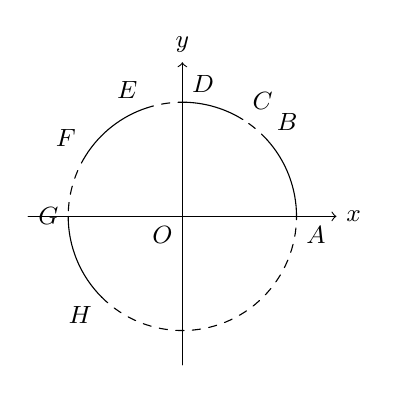
\begin{tikzpicture}[scale=1.45, font=\small, line cap=round]
  \draw[->] (-1.35,0)--(1.35,0) node[right] {$x$};
  \draw[->] (0,-1.3)--(0,1.35) node[above] {$y$};
  % 仅四段候选弧为实线；其余圆周分段画虚线
  \draw (1,0) arc (0:42:1);
  \draw[dashed] (42:1) arc (42:58:1);
  \draw (58:1) arc (58:88:1);
  \draw[dashed] (88:1) arc (88:108:1);
  \draw (108:1) arc (108:148:1);
  \draw[dashed] (148:1) arc (148:180:1);
  \draw (180:1) arc (180:225:1);
  \draw[dashed] (225:1) arc (225:360:1);
  \node[below left] at (0,0) {$O$};
  \node[below right] at (1,0) {$A$};
  \node[above right] at (42:1) {$B$};
  \node[above right] at (58:1) {$C$};
  \node[above right] at (0,1) {$D$};
  \node[above left] at (108:1) {$E$};
  \node[above left] at (148:1) {$F$};
  \node[left] at (180:1) {$G$};
  \node[below left] at (225:1) {$H$};
\end{tikzpicture}
\end{center}
\nopagebreak[4]
（A）$\widehat{AB}$　（B）$\widehat{CD}$　（C）$\widehat{EF}$　（D）$\widehat{GH}$

\Needspace{4\baselineskip}
\textbf{解析}

\Needspace{5\baselineskip}
按象限排除：第一象限中 $\tan\alpha>\sin\alpha$，与题设不符；第三象限 $\tan\alpha>0>\cos\alpha$，不符；第四象限 $\sin\alpha<0<\cos\alpha$，也不符。第二象限则可能满足。以 $\alpha=120^\circ$ 为例，
\nopagebreak[4]
\[
\tan\alpha=-\sqrt3<\cos\alpha=-\frac12<\sin\alpha=\frac{\sqrt3}{2}.
\]
该角的终边落在图中第二象限弧段 $\widehat{EF}$ 内，因此 $P$ 所在弧为 $\widehat{EF}$。

\gkanswer{答案：C}

\end{answer}
\begin{answer}
\gksolhead{8}{}

\textbf{题目}：

设集合 $A=\{(x,y)\mid x-y\ge1,\ ax+y>4,\ x-ay\le2\}$，则\mbox{（　　）}

（A）对任意实数 $a$，$(2,1)\in A$　（B）对任意实数 $a$，$(2,1)\notin A$

（C）当且仅当 $a<0$ 时，$(2,1)\notin A$　（D）当且仅当 $a\le\dfrac32$ 时，$(2,1)\notin A$

\Needspace{4\baselineskip}
\textbf{解析}

\Needspace{5\baselineskip}
将 $(2,1)$ 代入三个条件：第一式为 $2-1\ge1$，恒成立；第二式要求 $2a+1>4$，即 $a>3/2$；第三式为 $2-a\le2$，即 $a\ge0$。因此
\nopagebreak[4]
\[
(2,1)\in A\iff a>\frac32,
\]
等价地，对任意实数 $a$，$(2,1)\notin A$ 当且仅当 $a\le3/2$。

\gkanswer{答案：D}

\end{answer}
\gkpart{二、填空题}

\begin{answer}
\gksolhead{9}{}

\textbf{题目}：

设向量 $\boldsymbol a=(1,0)$，$\boldsymbol b\;(-1,m)$。若 $\boldsymbol a\perp(m\boldsymbol a-\boldsymbol b)$，则 $m=$\gkblank{}。

\begin{gktip}
第9题固定源在 $\boldsymbol b$ 与 $(-1,m)$ 之间未印等号；此处保留原貌，待核。
\end{gktip}

\Needspace{4\baselineskip}
\textbf{解析}

\Needspace{5\baselineskip}
固定源印作“$\boldsymbol b\;(-1,m)$”，在 $\boldsymbol b$ 与坐标对之间未见等号。\textbf{以下仅在假设题意为 $\boldsymbol b=(-1,m)$ 时推导}：
\nopagebreak[4]
\[
m\boldsymbol a-\boldsymbol b=(m,0)-(-1,m)=(m+1,-m).
\]
与 $\boldsymbol a=(1,0)$ 垂直，点积为 $m+1=0$，所以该假设下 $m=-1$。

若缺失等号确为排版遗漏，则 $m=-1$；题面原文及答案待核。

\gkanswer{答案：待核；若 $\boldsymbol b=(-1,m)$，则 $m=-1$}

\end{answer}
\begin{answer}
\gksolhead{10}{}

\textbf{题目}：

已知直线 $l$ 过点 $(1,0)$ 且垂直于 $x$ 轴。若 $l$ 被抛物线 $y^2=4ax$ 截得的线段长为 $4$，则抛物线的焦点坐标为\gkblank{}。

\Needspace{4\baselineskip}
\textbf{解析}

直线 $x=1$ 与抛物线 $y^2=4ax$ 的交点纵坐标为 $y=\pm2\sqrt a$（需 $a>0$），截线长度为 $4\sqrt a=4$，故 $a=1$。焦点坐标为 $(a,0)=(1,0)$。

\gkanswer{答案：$(1,0)$}

\end{answer}
\begin{answer}
\gksolhead{11}{}

\textbf{题目}：

能说明“若 $a>b$，则 $\dfrac1a<\dfrac1b$”为假命题的一组 $a,b$ 的值依次为\gkblank{}。

\Needspace{4\baselineskip}
\textbf{解析}

例如取 $a=1,b=-1$，则 $a>b$，但 $1/a=1>-1=1/b$，不满足所述结论，故命题为假。

\gkanswer{答案：例如 $a=1,b=-1$}

\end{answer}
\begin{answer}
\gksolhead{12}{}

\textbf{题目}：

若双曲线 $\dfrac{x^2}{a^2}-\dfrac{y^2}{4}=1\ (a>0)$ 的离心率为 $\dfrac{\sqrt5}{2}$，则 $a=$\gkblank{}。

\Needspace{4\baselineskip}
\textbf{解析}

\Needspace{5\baselineskip}
双曲线中 $c^2=a^2+4$，离心率 $c/a=\sqrt5/2$。平方得
\nopagebreak[4]
\[
\frac{a^2+4}{a^2}=\frac54\quad\Longrightarrow\quad a^2=16.
\]
因 $a>0$，$a=4$。

\gkanswer{答案：$4$}

\end{answer}
\begin{answer}
\gksolhead{13}{}

\textbf{题目}：

若 $x,y$ 满足 $x+1\le y\le2x$，则 $2y-x$ 的最小值是\gkblank{}。

\Needspace{4\baselineskip}
\textbf{解析}

\Needspace{5\baselineskip}
由 $x+1\le y\le2x$ 可知 $x+1\le2x$，即 $x\ge1$。又
\nopagebreak[4]
\[
2y-x\ge2(x+1)-x=x+2\ge3.
\]
在 $(x,y)=(1,2)$ 时满足约束且取到 $3$，故最小值为 $3$。

\gkanswer{答案：$3$}

\end{answer}
\begin{answer}
\gksolhead{14}{}

\textbf{题目}：

若 $\triangle ABC$ 的面积为 $\dfrac{\sqrt3}{4}(a^2+c^2-b^2)$，且 $\angle C$ 为钝角，则 $\angle B=$\gkblank{}；$\dfrac ca$ 的取值范围是\gkblank{}。

\Needspace{4\baselineskip}
\textbf{解析}

\Needspace{5\baselineskip}
设三角形边长 $a,b,c$ 分别对角 $A,B,C$。由面积表达式及正弦面积公式，
\nopagebreak[4]
\[
\frac12ac\sin B=\frac{\sqrt3}{4}(a^2+c^2-b^2).
\]
余弦定理给出 $a^2+c^2-b^2=2ac\cos B$，因此 $\sin B=\sqrt3\cos B$。又 $C$ 为钝角，故 $A+B<\pi/2$，特别地 $B$ 为锐角，于是 $B=\pi/3$。

\Needspace{5\baselineskip}
再由余弦定理对 $C$：$c^2=a^2+b^2-2ab\cos C$，$C$ 钝角等价于 $c^2>a^2+b^2$。而上面的面积条件和 $B=\pi/3$ 还给出
\nopagebreak[4]
\[
a^2+c^2-b^2=\frac{2ac}{\sqrt3}\sin\frac\pi3=ac,
\quad b^2=a^2+c^2-ac.
\]
\Needspace{5\baselineskip}
代入钝角条件，化为 $c^2>a^2+a^2+c^2-ac$，即 $c>2a$。反过来该不等式也推出 $C$ 钝，故
\nopagebreak[4]
\[
\frac ca>2.
\]

\gkanswer{答案：$\angle B=\pi/3$；$c/a>2$}

\end{answer}
\gkpart{三、解答题}

\begin{answer}
\gksolhead{15}{}

\textbf{题目}：

设 $\{a_n\}$ 是等差数列，且 $a_1=\ln2$，$a_2+a_3=5\ln2$。

（1） 求 $\{a_n\}$ 的通项公式；

（2） 求 $\mathrm e^{a_1}+\mathrm e^{a_2}+\cdots+\mathrm e^{a_n}$。

\Needspace{4\baselineskip}
\textbf{解析}

\textbf{(1) 解析}

\Needspace{5\baselineskip}
等差数列公差记为 $d$。由 $a_1=\ln2$，有 $a_2=\ln2+d$、$a_3=\ln2+2d$。条件给出
\nopagebreak[4]
\[
2\ln2+3d=5\ln2\quad\Longrightarrow\quad d=\ln2.
\]
所以 $a_n=\ln2+(n-1)\ln2=n\ln2$。

\textbf{(2) 解析}

\Needspace{5\baselineskip}
于是 $\mathrm e^{a_k}=2^k$，从而
\nopagebreak[4]
\[
\sum_{k=1}^n\mathrm e^{a_k}=2+2^2+\cdots+2^n=2^{n+1}-2.
\]

\gkanswer{答案（1）：$a_n=n\ln2$}

\gkanswer{答案（2）：$2^{n+1}-2$}

\end{answer}
\begin{answer}
\gksolhead{16}{}

\textbf{题目}：

已知函数 $f(x)=\sin^2x+\sqrt3\sin x\cos x$。

（1） 求 $f(x)$ 的最小正周期；

（2） 若 $f(x)$ 在区间 $\left[-\dfrac\pi3,m\right]$ 上的最大值为 $\dfrac32$，求 $m$ 的最小值。

\Needspace{4\baselineskip}
\textbf{解析}

\textbf{(1) 解析}

\Needspace{5\baselineskip}
用二倍角公式化简：
\nopagebreak[4]
\[
f(x)=\frac{1-\cos2x}{2}+\frac{\sqrt3}{2}\sin2x
=\frac12+\sin\left(2x-\frac\pi6\right).
\]
故最小正周期为 $\pi$。

\textbf{(2) 解析}

\Needspace{5\baselineskip}
函数最大值 $3/2$ 在
\nopagebreak[4]
\[
2x-\frac\pi6=\frac\pi2+2k\pi,
\quad x=\frac\pi3+k\pi
\]
处取得。左端点 $x=-\pi/3$ 对应相位 $-5\pi/6$。随着 $x$ 增大，函数在相位从 $-5\pi/6$ 到 $\pi/2$ 期间先降至 $-1/2$，再升至 $3/2$；此区间的最大值首次达到 $3/2$ 于 $x=\pi/3$。故使区间最大值为 $3/2$ 的最小右端点为 $m=\pi/3$。

\gkanswer{答案（1）：$\pi$}

\gkanswer{答案（2）：$m_{\min}=\pi/3$}

\end{answer}
\begin{answer}
\gksolhead{17}{}

\textbf{题目}：

电影公司随机收集了电影的有关数据，经分类整理得到下表：

\begin{center}
\begin{tabular}{crrrrrr}
\toprule
电影类型 & 第一类 & 第二类 & 第三类 & 第四类 & 第五类 & 第六类 \\
\midrule
电影部数 & 140 & 50 & 300 & 200 & 800 & 510 \\
好评率 & 0.4 & 0.2 & 0.15 & 0.25 & 0.2 & 0.1 \\
\bottomrule
\end{tabular}
\end{center}

好评率是指：一类电影中获得好评的部数与该类电影的部数的比值。

（1） 从电影公司收集的电影中随机选取 1 部，求这部电影是获得好评的第四类电影的概率；

（2） 随机选取 1 部电影，估计这部电影没有获得好评的概率；

（3） 电影公司为增加投资回报，拟改变投资策略，这将导致不同类型电影的好评率发生变化。假设表格中只有两类电影的好评率数据发生变化，那么哪类电影的好评率增加 0.1，哪类电影的好评率减少 0.1，使得获得好评的电影总部数与样本中的电影总部数的比值达到最大？（只需写出结论）

\Needspace{4\baselineskip}
\textbf{解析}

总电影数为 $140+50+300+200+800+510=2000$。

\textbf{(1) 解析} 第四类好评数为 $200\times0.25=50$，概率为 $50/2000=1/40$。

\textbf{(2) 解析} 各类好评数依次为 $56,10,45,50,160,51$，合计 $372$；未获好评的概率估计为 $(2000-372)/2000=407/500$。

\textbf{(3) 解析} 净增好评数为 $0.1$ 乘以两类电影部数之差；选数量最多的第五类（800部）增加，数量最少的第二类（50部）减少。

\gkanswer{答案（1）：$1/40$}

\gkanswer{答案（2）：$407/500$}

\gkanswer{答案（3）：第五类增加、第二类减少}

\end{answer}
\begin{answer}
\gksolhead{18}{}

\textbf{题目}：

如图，在四棱锥 $P-ABCD$ 中，底面 $ABCD$ 为矩形，平面 $PAD\perp$ 平面 $ABCD$，$PA\perp PD$，$PA=PD$，$E,F$ 分别为 $AD,PB$ 的中点。
\nopagebreak[4]
\begin{center}% 2018 北京卷文第18题：四棱锥与中点（据固定源第1064页重绘）
\begin{tikzpicture}[font=\small, line cap=round, line join=round]
  % 投影位置按原图透视关系布置
  \coordinate (A) at (0,0);
  \coordinate (B) at (1.5,-0.35);
  \coordinate (C) at (4.2,0.05);
  \coordinate (D) at (2.7,0.55);
  \coordinate (P) at (1.25,3.0);
  \coordinate (E) at ($(A)!0.5!(D)$);
  \coordinate (F) at ($(P)!0.5!(B)$);
  % 矩形底面：后边 AD、DC 为虚线，前侧为实线
  \draw (A)--(B)--(C);
  \draw[dashed] (C)--(D)--(A);
  % 侧棱：遮挡棱以虚线表示
  \draw (P)--(A) (P)--(B) (P)--(C);
  \draw[dashed] (P)--(D);
  % 原图标示 P--E 为虚线；不绘制 E--F
  \draw[dashed] (P)--(E);
  \fill (A) circle (1.1pt) (B) circle (1.1pt) (C) circle (1.1pt) (D) circle (1.1pt)
        (P) circle (1.1pt) (E) circle (1.1pt) (F) circle (1.1pt);
  \node[above] at (P) {$P$};
  \node[left] at (A) {$A$};
  \node[below] at (B) {$B$};
  \node[right] at (C) {$C$};
  \node[right] at (D) {$D$};
  \node[below left] at (E) {$E$};
  \node[right] at (F) {$F$};
\end{tikzpicture}
\end{center}
\nopagebreak[4]
（1） 求证：$PE\perp BC$；

（2） 求证：平面 $PAB\perp$ 平面 $PCD$；

（3） 求证：$EF\parallel$ 平面 $PCD$。

\Needspace{4\baselineskip}
\textbf{解析}

\textbf{(1) 解析} $PA=PD$，$E$ 为 $AD$ 中点，故 $PE\perp AD$。两平面垂直且交线为 $AD$，所以 $PE\perp$ 底面 $ABCD$，从而 $PE\perp BC$。

\textbf{(2) 解析} 矩形给出 $AB\perp AD$，且 $AB\perp PE$，故 $AB\perp$ 平面 $PAD$，特别地 $AB\perp PD$。又 $PA\perp PD$，所以 $PD\perp$ 平面 $PAB$。由 $PD\subset$ 平面 $PCD$，得平面 $PAB\perp$ 平面 $PCD$。

\Needspace{5\baselineskip}
\textbf{(3) 解析} 取 $A=(0,0,0)$，$D=(d,0,0)$，$B=(0,w,0)$，则 $P=(d/2,0,d/2)$。于是 $E=(d/2,0,0)$、$F=(d/4,w/2,d/4)$，且
\nopagebreak[4]
\[
\overrightarrow{EF}=(-d/4,w/2,d/4)
=\tfrac12\overrightarrow{DC}-\tfrac12\overrightarrow{PD}.
\]
因此 $EF$ 的方向平行于平面 $PCD$；$E$ 不在该平面上，故 $EF\parallel$ 平面 $PCD$。

\gkanswer{答案（1）：成立}

\gkanswer{答案（2）：成立}

\gkanswer{答案（3）：成立}

\end{answer}
\begin{answer}
\gksolhead{19}{}

\textbf{题目}：

设函数 $f(x)=[ax^2-(3a+1)x+3a+2]\mathrm e^x$。

（1） 若曲线 $y=f(x)$ 在点 $(2,f(2))$ 处的切线斜率为 $0$，求 $a$；

（2） 若 $f(x)$ 在 $x=1$ 处取得极小值，求 $a$ 的取值范围。

\Needspace{4\baselineskip}
\textbf{解析}

\Needspace{5\baselineskip}
令 $g(x)=ax^2-(3a+1)x+3a+2$，则 $f(x)=g(x)\mathrm e^x$，从而
\nopagebreak[4]
\[
f'(x)=(g(x)+g'(x))\mathrm e^x=(ax^2-(a+1)x+1)\mathrm e^x=(x-1)(ax-1)\mathrm e^x.
\]

\textbf{(1) 解析}

在 $x=2$ 处切线斜率为零，且 $\mathrm e^2>0$，故 $(2-1)(2a-1)=0$，得 $a=1/2$。

\textbf{(2) 解析}

要 $f$ 在 $x=1$ 处取得极小值，导数须在 $1$ 左侧为负、右侧为正。$f'(x)$ 的符号由 $(x-1)(ax-1)$ 决定。若 $a>1$，则 $1/a<1$，在 $x=1$ 左右邻域内 $ax-1>0$，导数随 $(x-1)$ 变号，负变正，满足极小值条件。若 $a<1$，则 $1/a$（当 $a>0$）在 1 的右侧，或 $a\le0$ 时 $ax-1$ 在 1 邻域保持负，导数在 1 处均为正变负或不变号，不产生极小值。$a=1$ 时 $f'(x)=(x-1)^2\mathrm e^x\ge0$，不变号。因此 $a>1$。

\gkanswer{答案（1）：$a=1/2$}

\gkanswer{答案（2）：$a>1$}

\end{answer}
\begin{answer}
\gksolhead{20}{}

\textbf{题目}：

已知椭圆 $M:\dfrac{x^2}{a^2}+\dfrac{y^2}{b^2}=1\ (a>b>0)$ 的离心率为 $\dfrac{\sqrt6}{3}$，焦距为 $2\sqrt2$，斜率为 $k$ 的直线 $l$ 与椭圆 $M$ 有两个不同的交点 $A,B$。

（1） 求椭圆 $M$ 的方程；

（2） 若 $k=1$，求 $|AB|$ 的最大值；

（3） 设 $P(-2,0)$，直线 $PA$ 与椭圆 $M$ 的另一个交点为 $C$，直线 $PB$ 与椭圆 $M$ 的另一个交点为 $D$。若 $C,D$ 和点 $Q\left(-\dfrac74,\dfrac14\right)$ 共线，求 $k$。

\Needspace{4\baselineskip}
\textbf{解析}

\textbf{(1) 解析}

\Needspace{5\baselineskip}
焦距为 $2\sqrt2$，故焦半距 $c=\sqrt2$。离心率 $c/a=\sqrt6/3$，得 $a=\sqrt3$，$a^2=3$；又 $b^2=a^2-c^2=1$。椭圆为
\nopagebreak[4]
\[
\frac{x^2}{3}+y^2=1.
\]

\textbf{(2) 解析}

\Needspace{5\baselineskip}
令直线斜率为 1，写作 $y=x+h$。代入椭圆得
\nopagebreak[4]
\[
\frac{x^2}{3}+(x+h)^2=1.
\]
\Needspace{5\baselineskip}
两交点弦长满足 $|AB|=\sqrt{1+1}\,|x_1-x_2|$。二次方程判别式化简可得
\nopagebreak[4]
\[
(x_1-x_2)^2=\frac{12(4-h^2)}{16}=\frac34(4-h^2),\quad |AB|^2=\frac32(4-h^2)\le6.
\]
等号在 $h=0$ 时取到，故最大值为 $\sqrt6$。

\textbf{(3) 解析} 设 $AB$ 为 $y=kx+h$。对椭圆点 $X=(x,y)$，过 $P=(-2,0)$ 的另一交点 $X'=P+\lambda(X-P)$；代入椭圆并利用 $X$ 在椭圆上，得 $\lambda=1/(4x+7)$，分母在椭圆上为正。

\Needspace{5\baselineskip}
记 $z=1/(4x+7)$，结合 $y=kx+h$，有
\nopagebreak[4]
\[
X'_x=-\frac74+\frac z4,\qquad
X'_y=\frac{k}{4}+\left(h-\frac{7k}{4}\right)z.
\]
$C,D$ 对应的 $z$ 值不同；$Q=(-7/4,1/4)$ 与它们共线当且仅当 $k/4=1/4$，故 $k=1$。取 $h=0$ 时直线与椭圆有两个不同交点，故该值可取。

\gkanswer{答案（1）：$x^2/3+y^2=1$}

\gkanswer{答案（2）：$\sqrt6$}

\gkanswer{答案（3）：$k=1$}

\end{answer}